%!TEX root = ../ausarbeitung.tex
\section{Klassifizierung mit Histograms of Gradients und Support Vector Machines} \label{sec:HOG}


\subsection{Einführung zu Histograms of Oriented Gradients} \label{ssec:intro_HOG}

Die Bezeichnung \textit{Histograms of Oriented Gradients} (HOG) bezeichnet einen Feature-Deskriptor und wurde bekannt durch die Arbeit von Navneet Dalal und Bill Triggs \cite{dalal05}. Diese setzen den HOG-Deskriptor ein, um Fußgänger zu detektieren. Später wurde er auch für andere Objekte eingesetzt. Die Berechnung des HOG-Deskriptors lässt sich in drei Schritte unterteilen: Gradientenberechnung, Gruppierung der Orientierungen und Histogrammerzeugung. Häufig werden auch Vorverarbeitungsschritte, wie zum Beispiel ein Histogrammausgleich durchgeführt.

Zur Gradientenberechnung wird der Sobel-Operator verwendet. Eine visuelle Darstellung des Ergebnisses ist in Abbildung~\ref{fig:sobel} gezeigt. Zu sehen ist die Magnitude der Ableitung über die vertikale (links) und horizontale (rechts) Bildachse. Dabei entspricht in dieser Darstellung der Grauwert der positiv definierten Magnitude des Gradienten. Mit den folgenden Formeln lassen sich aus den beiden Gradientenbildern die positiv definierte Gesamtmagnitude $|G|$ und die Orientierung $\Theta$ berechnen:  

\begin{equation}
|G| = \sqrt{G_x^2 + G_y^2}
\end{equation}
\begin{equation}
\Theta = \arctan({G_x, G_y})
\end{equation}

\begin{center}
\begin{tabular}{c}
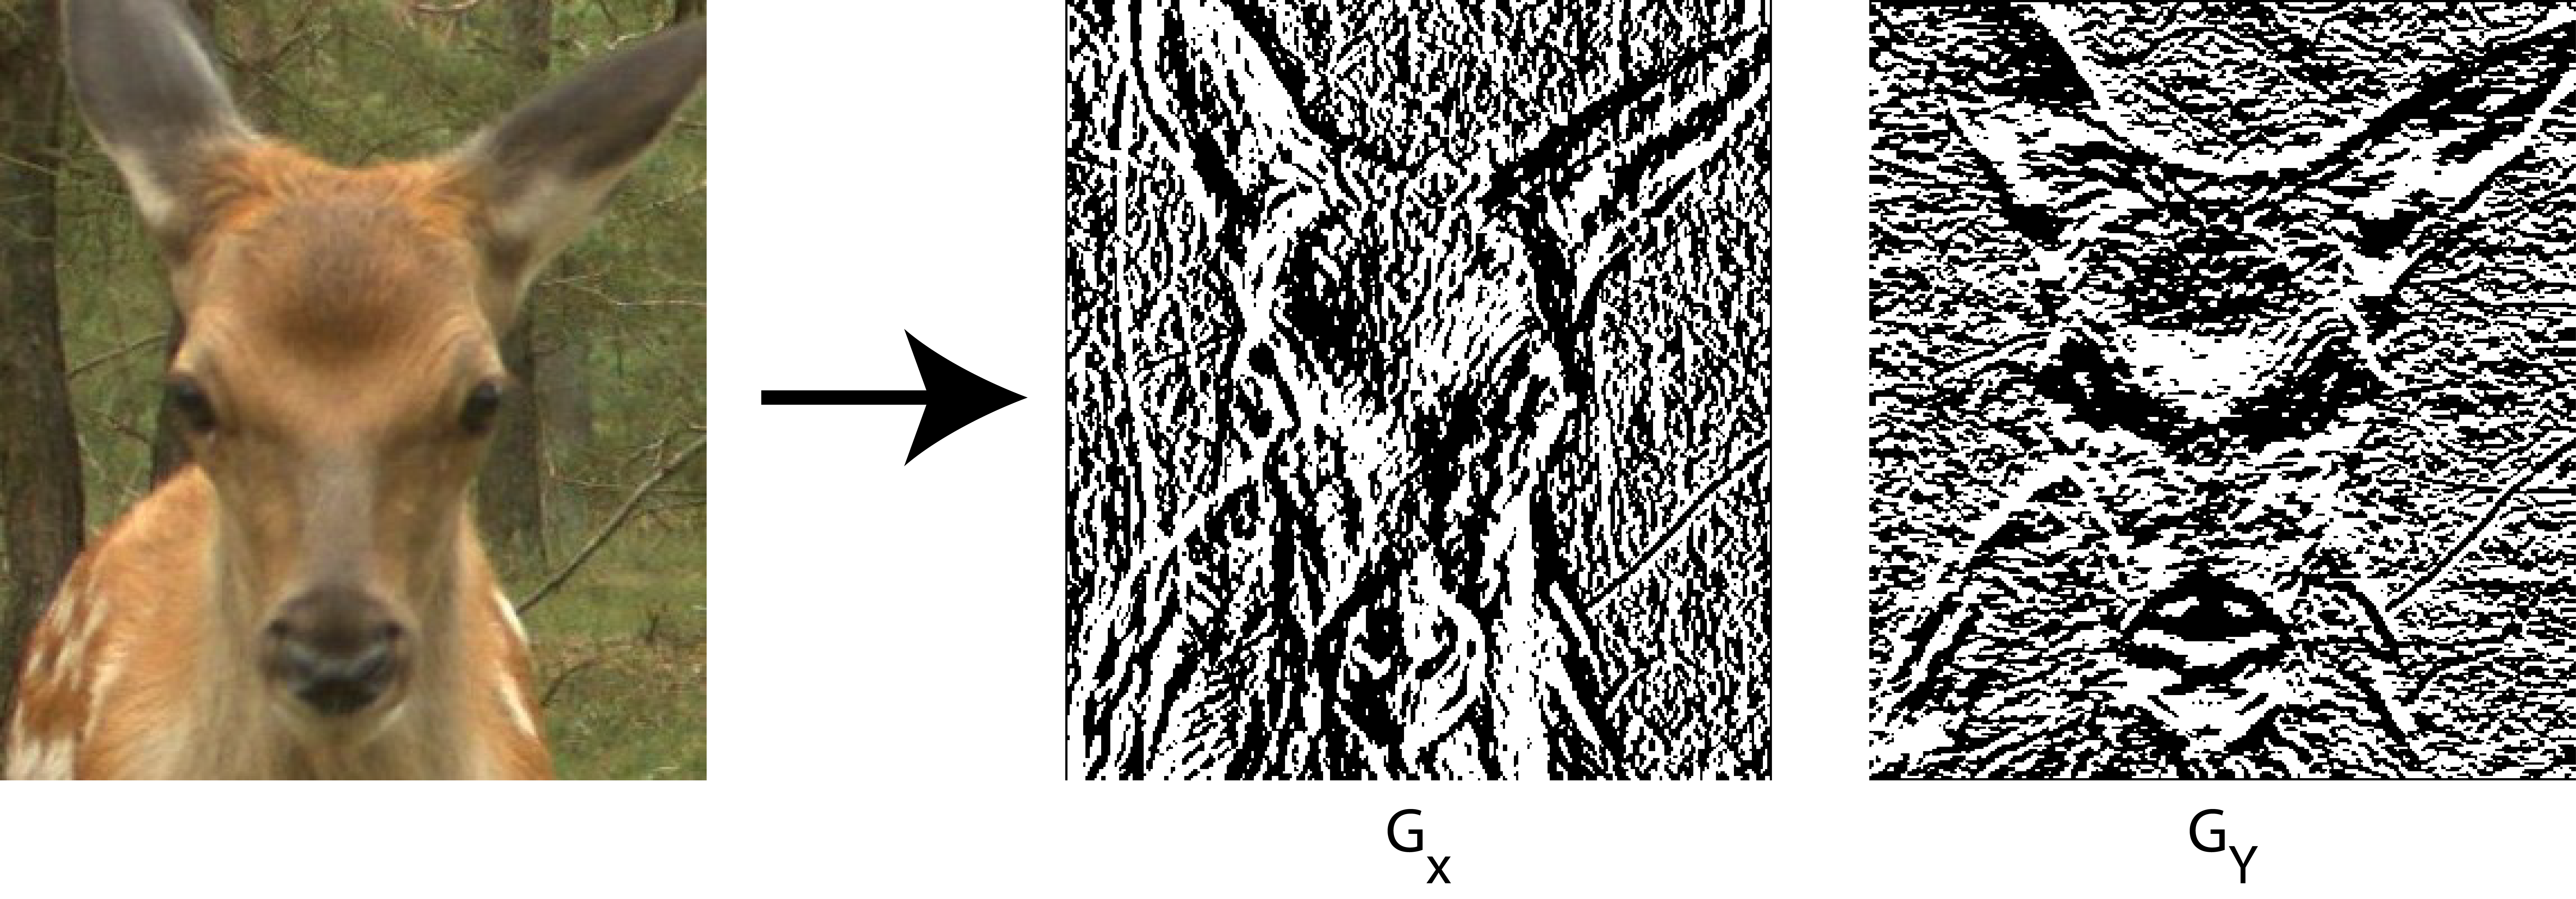
\includegraphics[trim={0 0cm 0cm 0cm},clip=true,width=13cm]{img/sobel.png}
\end{tabular}
\captionof{figure}{Exemplarische Ergebnisbilder des Sobel-Operators für die vertikale und horizontale Bildachse. Die Grauwerte entsprechen der Magnitude des Gradienten.}
\label{fig:sobel}
\end{center}

Für jeden Pixel eines Bildes werden die Magnitude und Orientierung berechnet. Anschließend werden sie entsprechend ihrer Orientierung in Gruppen sortiert. Häufig wird das Vorzeichen der Orientierung ignoriert und sie werden in neun Gruppen zusammengefasst. Durch das Ignorieren der Richtung wird also nur ein halber Kreis betrachtet (0 - 180°). Bei neun Gruppen bedeutet dies, dass jede Gruppe 20° abdeckt. Der Wert dieser Gruppe ist dann die Summe aller Magnituden der Pixel, die dieser Gruppe zugewiesen wurden. Es ist jedoch auch möglich andere Einteilungen zu verwenden. \\
Formal ist ein solches Histogramm aus neun Werten bereits ein HOG. Allerdings ist der Informationsgehalt dieser Repräsentation sehr gering. Um den Informationsgehalt zu erhöhen wird das Bild stattdessen systematisch in gleich große Bereiche unterteilt und für jeden Bereich ein Histogramm gebildet. Diese Histogramme werden abschließend konkateniert und als ein HOG-Deskriptor verwendet. Durch die Unterteilung werden Informationen der einzelnen Bildbereich bewahrt und somit kann ein Bild wesentlich besser beschrieben werden. \\
Die systematische Unterteilung des Bildes wird wie folgt durchgeführt. Das Bild wird in gleich große Zellen unterteilt, sodass jeder Pixel in genau einer Zelle enthalten ist (siehe Abbildung~\ref{fig:sobel2hog} rotes Raster). Anschließend werden jeweils vier dieser Zellen zu einem Block zusammengefasst (siehe Abbildung~\ref{fig:sobel2hog} grünes Rechteck) und für jeden dieser Blöcke wird nach dem \textit{Sliding-Window}-Prinzip ein Histogramm erstellt. Jedes dieser Histogramme wird anschließend normalisiert, um eine belichtungsunabhängige Repräsentation zu erhalten. Dies bedeutet dass jede Zelle - außer den Randzellen - viermal in einem Histogramm repräsentiert wird. Diese Methode wird angewendet, da so durch die Normalisierung alle lokalen Kontexte betrachtet werden und weniger Information durch die Normalisierung verloren geht. Das resultiert beispielsweise in einer erhöhten Invarianz zu Schatten im Bild. \\
Exemplarisch ist in Abbildung~\ref{fig:img2HOG} eine visuell aufbereitete Repräsentation eines HOG-Deskriptors gezeigt. In dieser Darstellung ist das gezeigte Reh noch zu erkennen, da der Deskriptor deutlich die Kanten des Tieres hervorhebt. Diese veranschaulicht, dass die essentiellen Informationen erhalten bleiben, obwohl die Datenmenge auf einen Bruchteil reduziert wurde. Um die Vergleichbarkeit der HOG-Deskriptoren zu gewährleisten, muss garantiert werden, dass die Deskriptoren dieselbe Dimension besitzen. Das wird erreicht, indem die betrachteten Bilder oder Bildausschnitte auf eine einheitliche Größe skaliert werden und anschließend das selbe Raster aus Zellen verwendet wird.  \cite{dalal05}\cite{HOG1}

\begin{center}
\begin{tabular}{c}
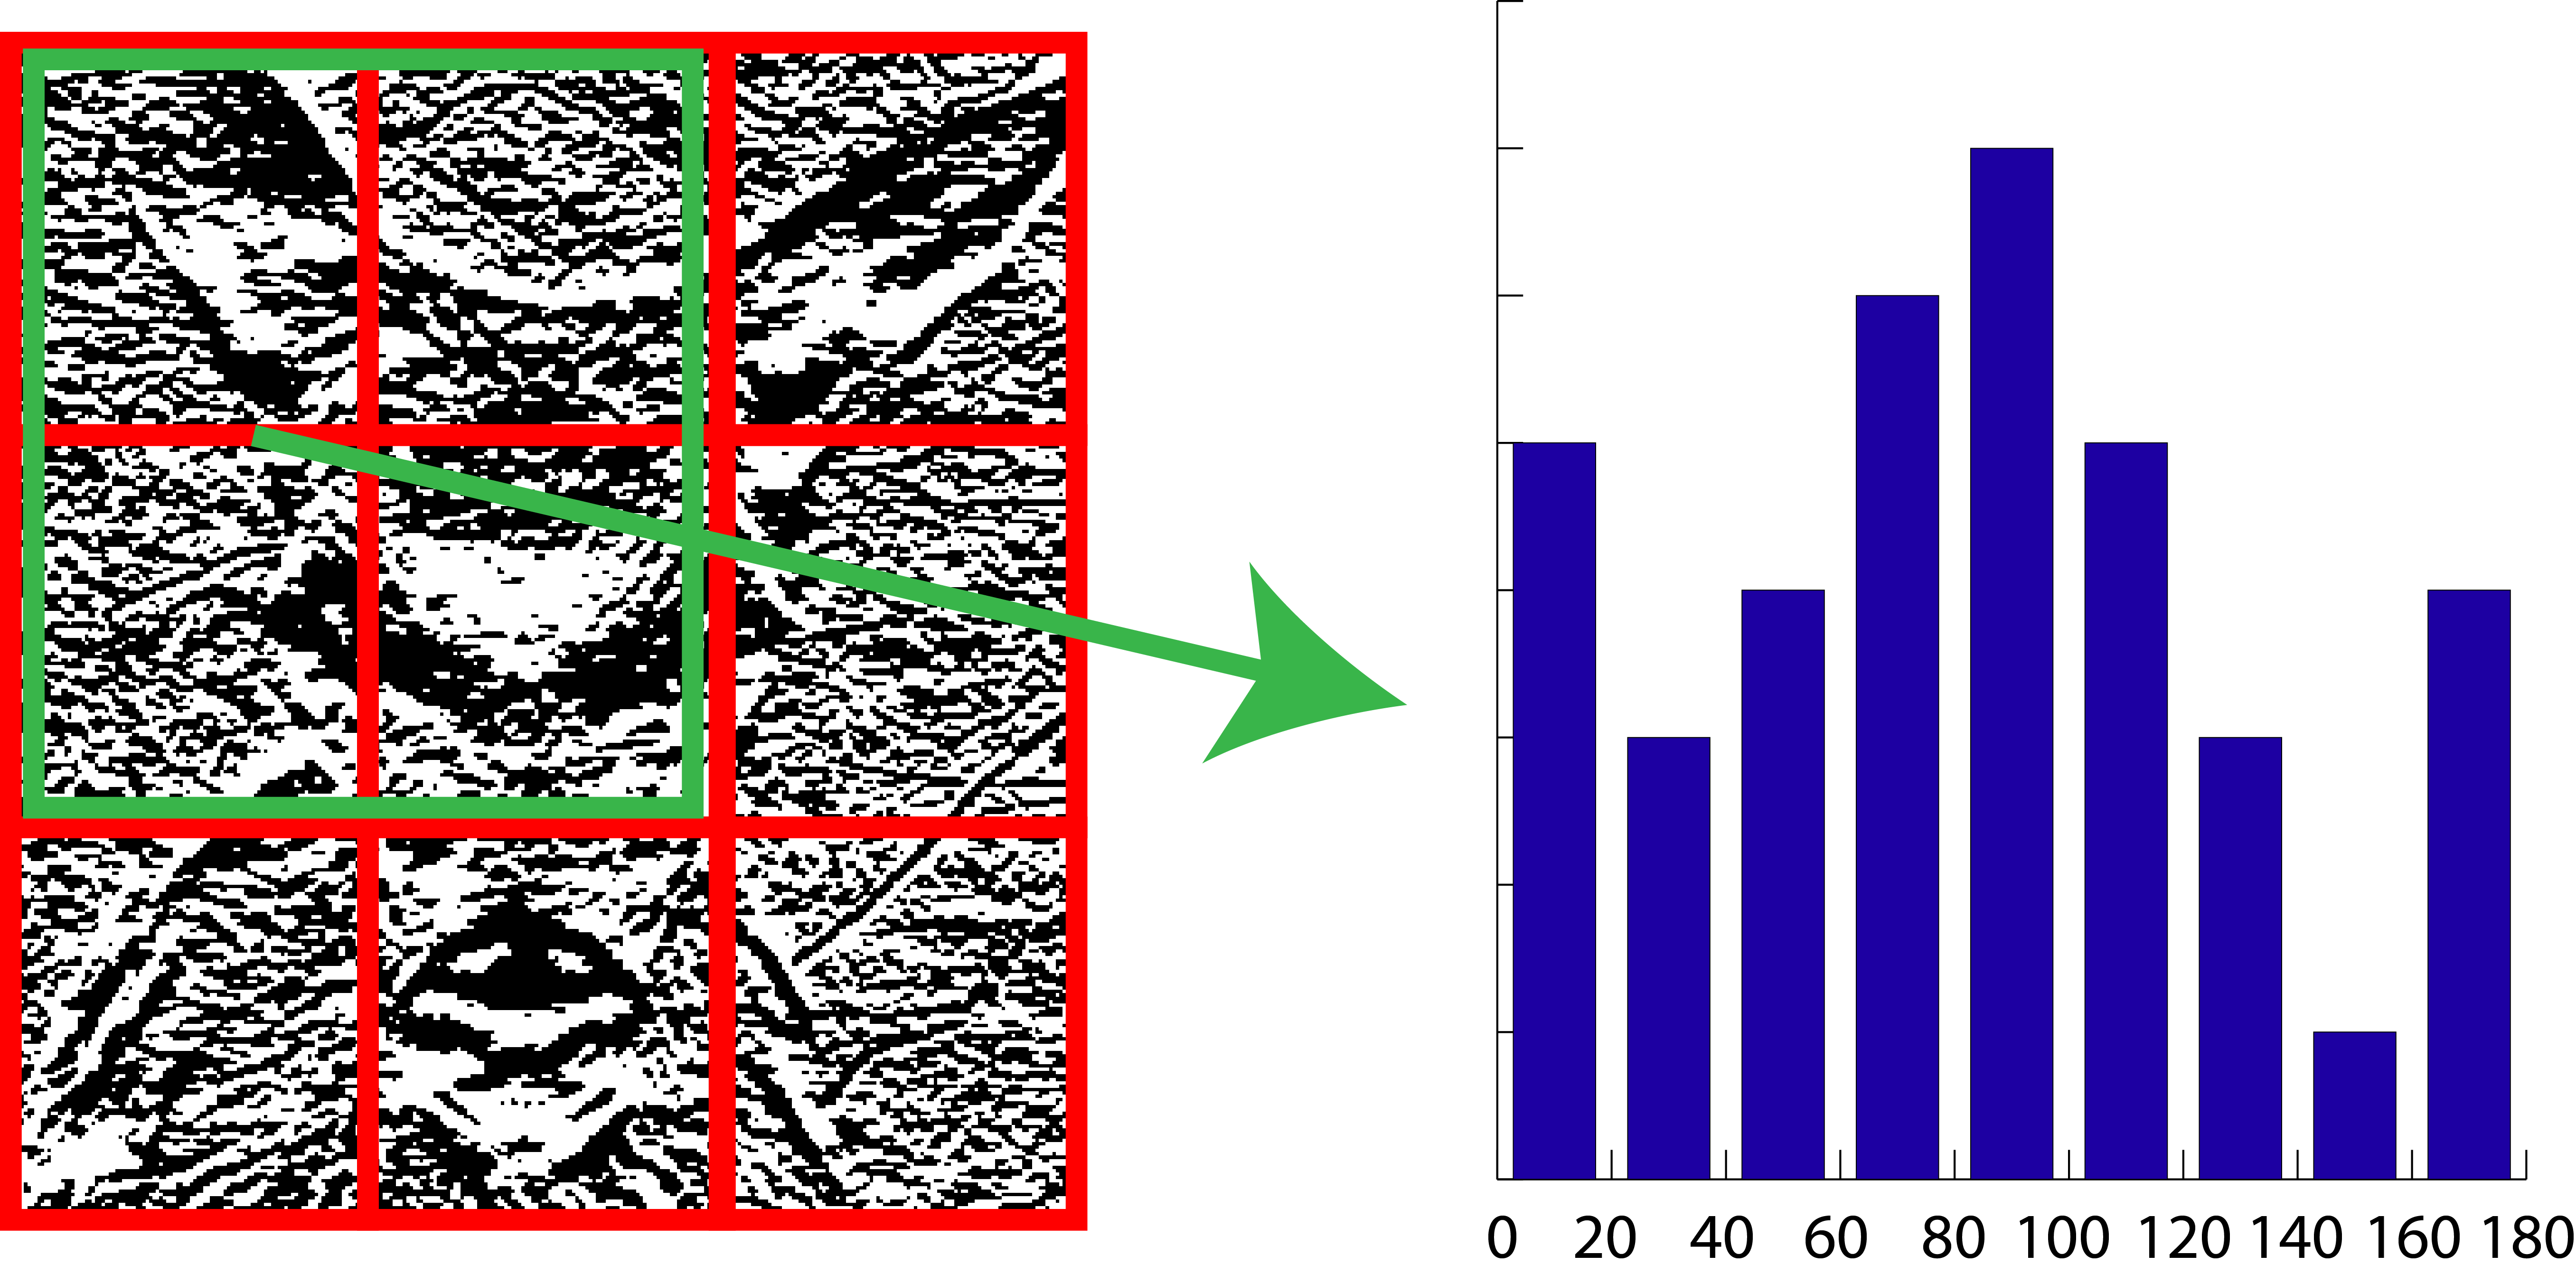
\includegraphics[trim={0 0cm 0cm 0cm},clip=true,width=13cm]{img/sobel2hog.png}
\end{tabular}
\captionof{figure}{Veranschaulichung der Erstellung eines HOG-Deskriptors. Das rote Raster visualisiert die Unterteilung in Zellen. Jeweils vier dieser Zellen werden zusammen als ein Block betrachtet, sodass hier vier Blöcke möglich wären. Für jeden Block wird anschließend ein normalisiertes Histogramm erstellt. Hier exemplarisch nur für den grünen Block gezeigt.}
\label{fig:sobel2hog}
\end{center}

\begin{center}
\begin{tabular}{c}
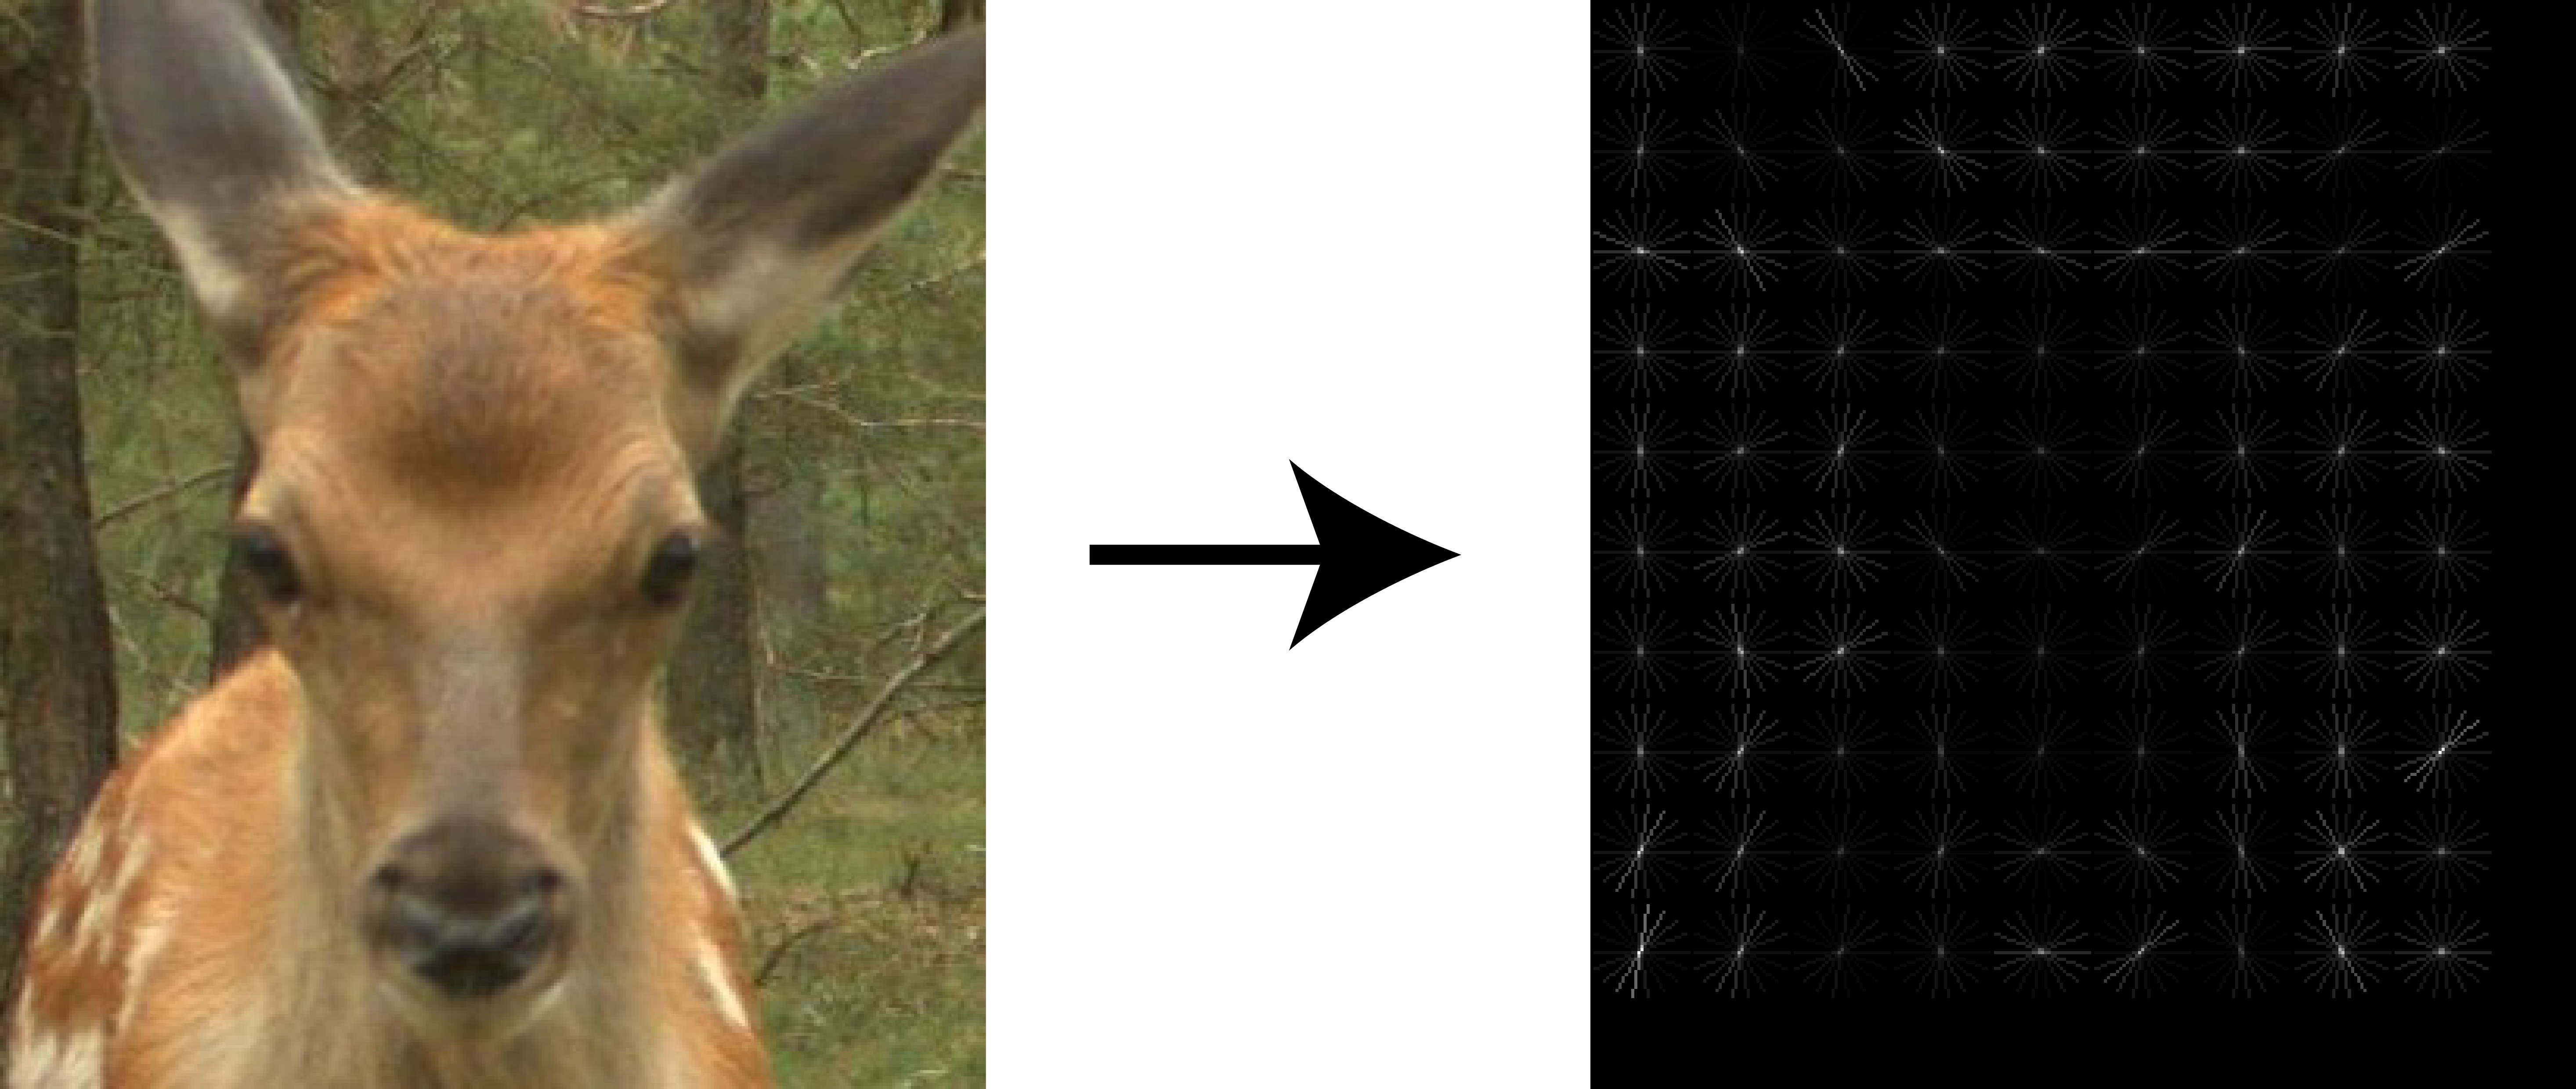
\includegraphics[trim={0 0cm 0cm 0cm},clip=true,width=13cm]{img/Img2HOG.png}
\end{tabular}
\captionof{figure}{Exemplarischer Bildausschnitt (links) und die visuell aufbereitete Repräsentation als HOG-Deskriptor (rechts). In der HOG-Repräsentation ist es immer noch möglich das Reh zu erkennen.}
\label{fig:img2HOG}
\end{center}


\subsection{Technische Umsetzung der Klassifizierung} \label{ssec:implementation}
Umgesetzt wurde der HOG-basierte Klassifizierer in Python mit OpenCV (Version: \texttt{opencv-contrib-python} 3.4.2.17). Der Klassifizierer setzt voraus, dass Bilder und die interessanten Regionen (ROI) bereits bestimmt wurden. Details zur ROI Bestimmungen werden in Kapitel~\ref{sec:PCA} gegeben. Eine Übersicht der Arbeitsweise wird in Abbildung~\ref{fig:hog_classification_ov} gezeigt. Dabei gibt es zwei Phasen: 1. Training und 2. Klassifikation. Die Trainings Phase wird durch den oberen Verlauf in der Abbildung skizziert. Zuerst werden aus einem gelabelten Bilddatensatz deren relevante ROIs selektiert. Für jedes ROI dieser Bilder wird, wie in Abschnitt~\ref{ssec:intro_HOG} erklärt, ein HOG-Deskriptor berechnet. Dabei wurde darauf geachtet, dass jedes ROI das selbe Seitenverhältnis besitzt. Zur Beschleunigung der Berechnung wurde die ROI nur als Graustufenbild verarbeitet und auf eine Größe von 64 x 128 Pixel² skaliert. Eine Zelle wurde auf 16 x 16 Pixel festgelegt, sodass eine Blockgröße von 32 x 32 Pixel² verwendet wurde. Diese Parametersatz wurde empirisch als der mit den Ergebnissen bestimmt (siehe Kapitel~\ref{sssec:HOG:parmeter}). Außerdem wurden die Orientierungen in neun Gruppen sortiert, sodass eine richtungsunabhängige Orientierung betrachtet wurde. Sonstige Parameter des HOG-Deskriptors wurden auf den entsprechenden Standardwerten der OpenCV-Implementierung belassen. 

Diese Deskriptoren sollen mit einer Support Vektor Machine (SVM) trainiert und im Anschluss klassifiziert werden. Dazu wurde die von OpenCV zur Verfügung gestellte Implementierung einer SVM verwendet. Als Kernel der SVM wurde eine radiale Basisfunktion gewählt. Experimentell wurden die Parameter $C = 12,5$ und $\gamma = 0,50625$ als optimal bestimmt. Details zur Parameterwahl werden im Kapitel~\ref{sssec:HOG:parmeter} beschrieben.\\
Mithilfe der so trainierten SVM kann dann in der 2. Phase die Klassifikation der Bilder durchgeführt werden. Dazu werden analog für Bildausschnitte der Testdaten Feature-Deskriptoren berechnet und diese von der SVM klassifiziert. Die Qualität dieser Klassifizierung wird im Unterkapitel \ref{sec:HOG_parameter_and_results} beschrieben.
\begin{center}
\begin{tabular}{c}
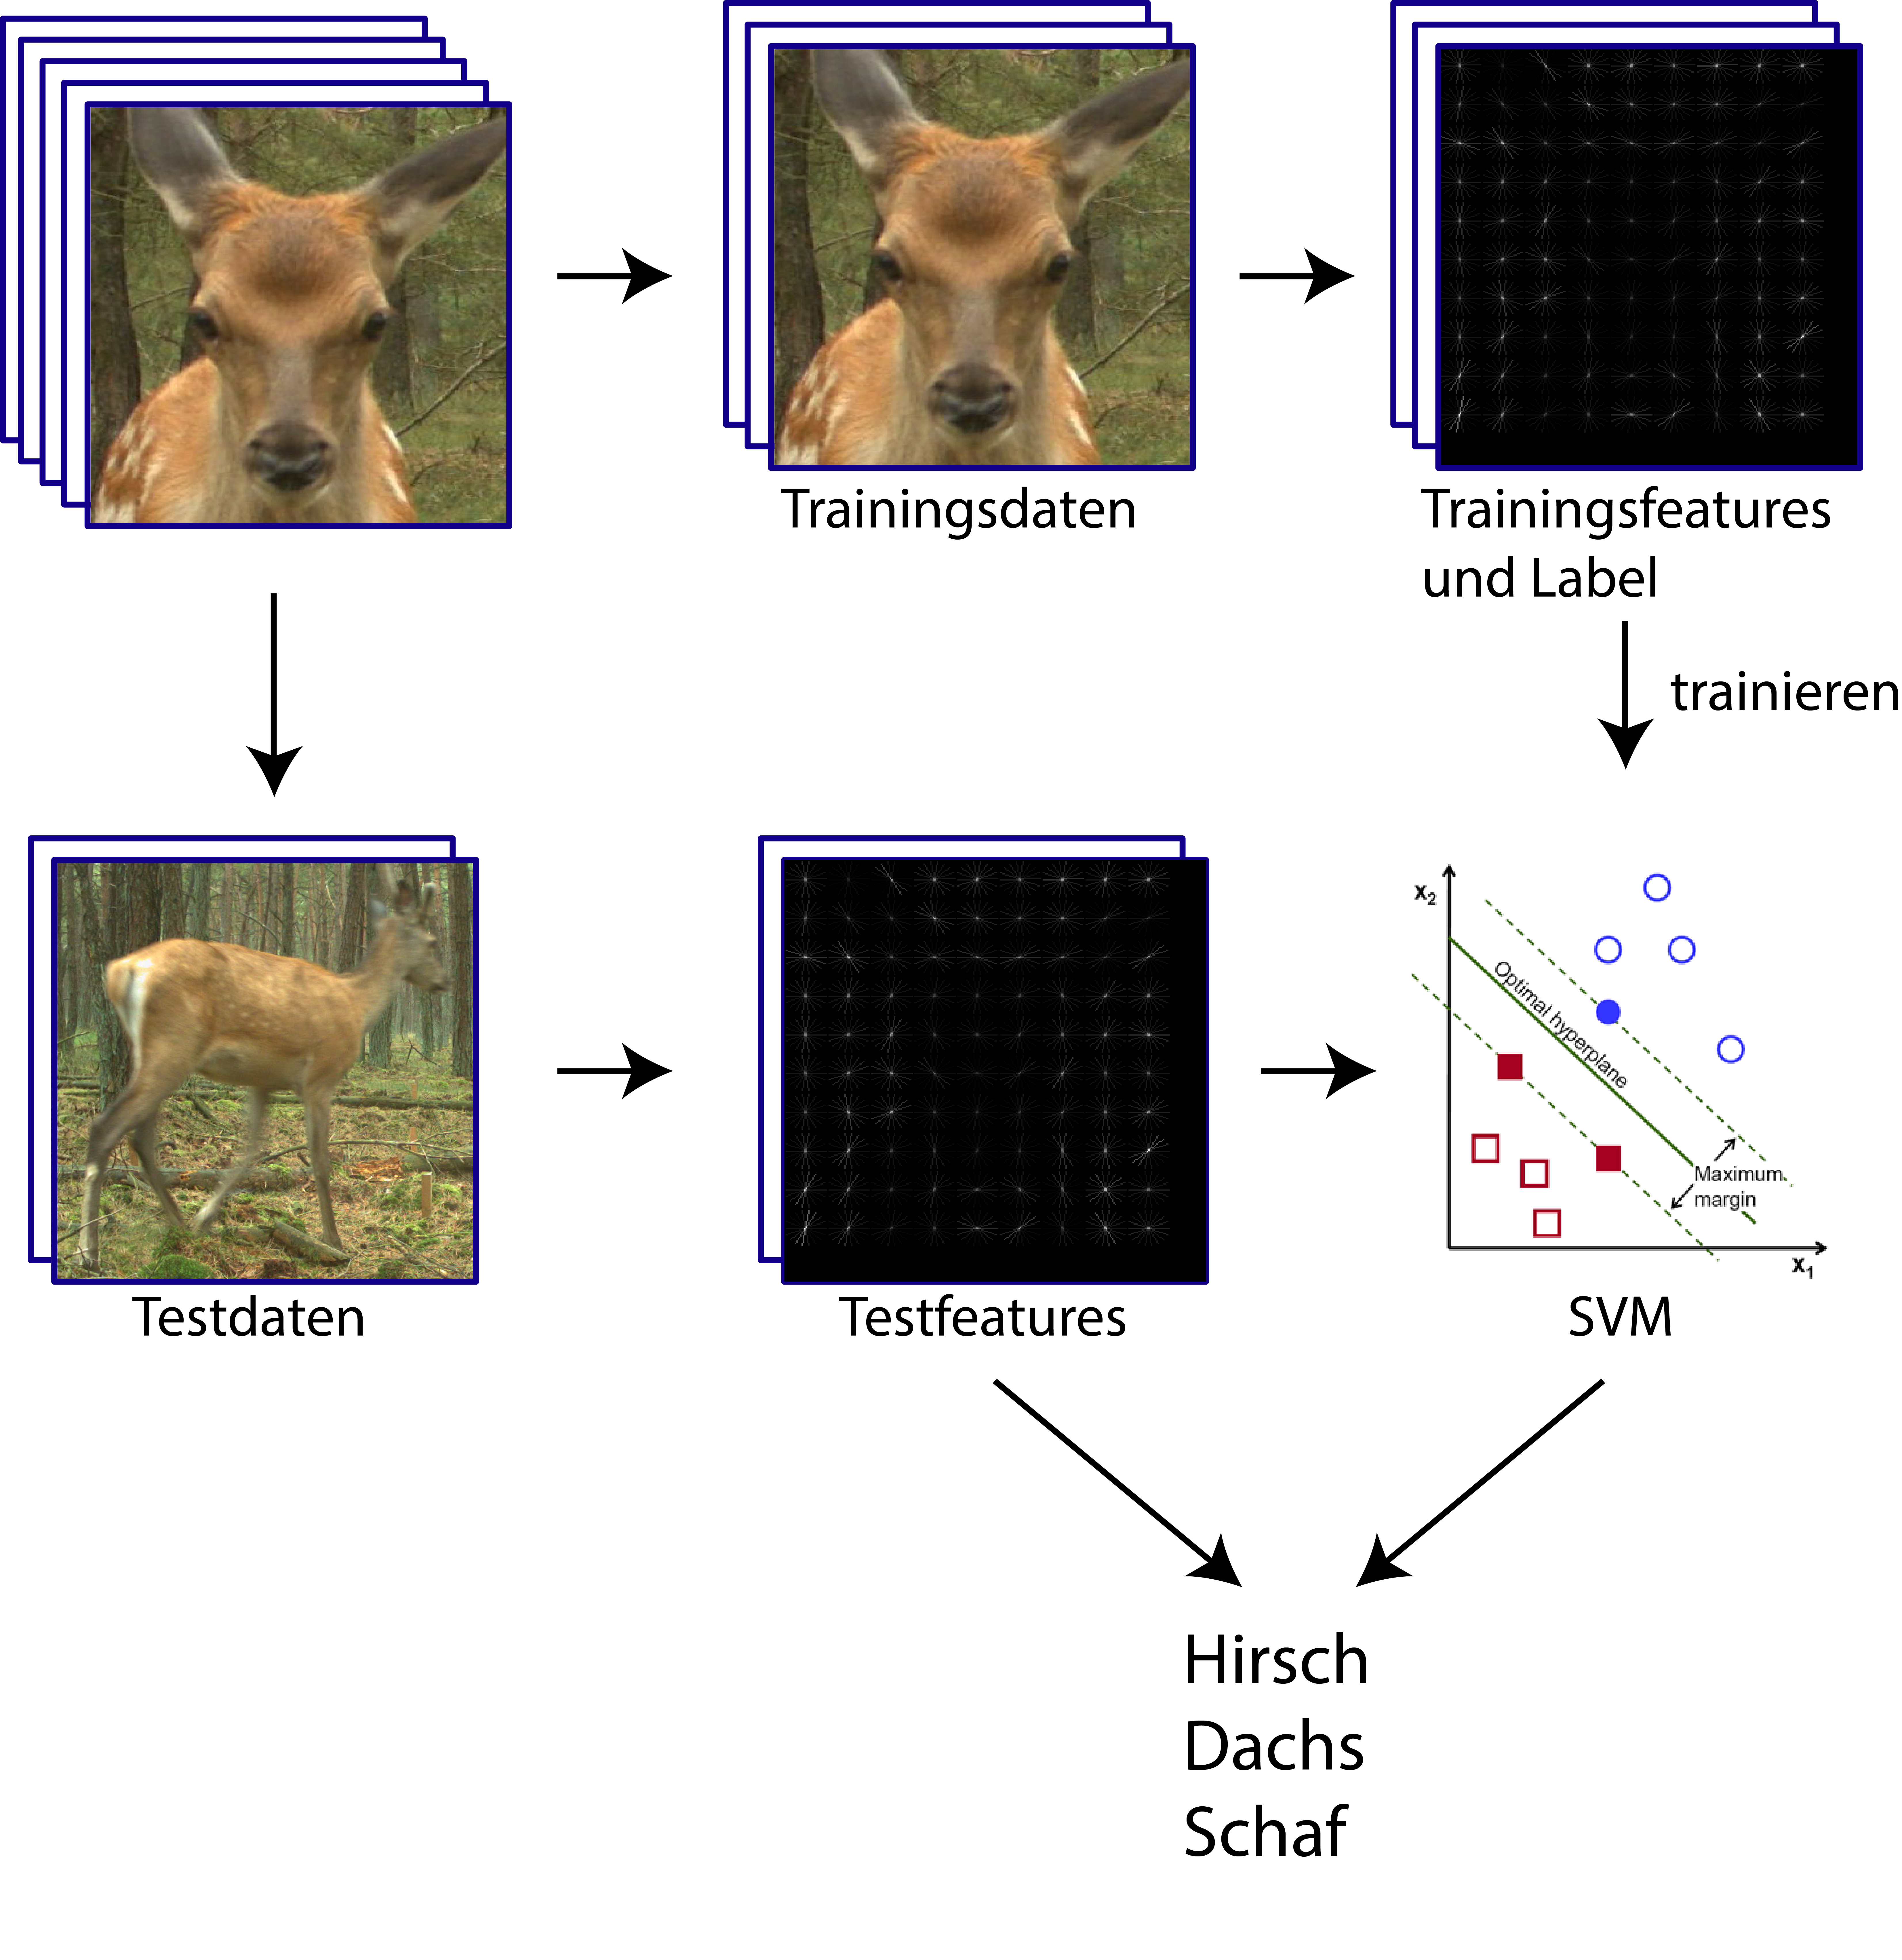
\includegraphics[trim={0 0cm 0cm 0cm},clip=true,width=10cm]{img/ClassificationOverview.png}
\end{tabular}
\captionof{figure}{Schaubild zur Klassifizierung mit einer SVM. Der obere Pfad repräsentiert die Trainings- und der untere die Klassifizierungsphase. (Das SVM Bild (rechts unten) wurde aus der OpenCV-Dokumentation übernommen \cite{SVM1})}
\label{fig:hog_classification_ov}
\end{center}
